\section{Use Cases}\label{sec:use-cases}

The following use cases further explain some of the problems that users of Smart Home solutions may encounter: 

\begin{quotation}\emph{\textbf{Use case: John}\\
John is enthusiastic about gadgets and new technology. He therefore owns a lot of \sdevs~from various manufacturers, and nearly all his electronics are connected to the Internet. John wants to put on a movie, turn on his surround sound, and dim the light. To do so he has to find and open the phone application for the television to turn it on. Next he has to find another application to dim the light. This application is connected to a \hub~that is connected to all of the lights in the living room, which allows him to dim them simultaneous. To fully enjoy the movie, he also wants to turn on his surround sound system. This requires that he finds the Wi-Fi connected controller for the surround system.}
\end{quotation}

\begin{figure}[H]
     \center{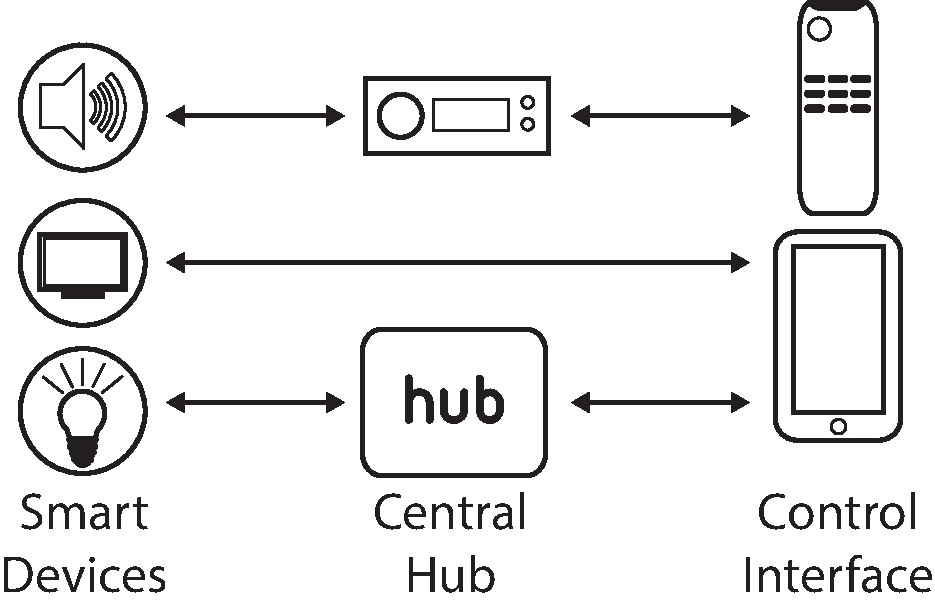
\includegraphics[width=\textwidth -200px]
     {graphics/smarthome-john.pdf}}
     \caption{\label{fig:use-case-1} Illustration of John's use case.}
\end{figure}

\begin{quotation}\emph{\textbf{Use case: Arthur}\\
Arthur likes to listen to music when he is at home. He has therefore purchased expensive built-in wireless speakers for every room. The speakers can only be controlled through a \hub~from a \phone. One day Arthur comes home from work and tries to turn on the music, but something is wrong - there is no sound from the speaker. After checking both the speakers and the wireless network without results, he discovers that the problem is that the \hub~is broken. He now has to wait for the \hub~to be repaired. This use case is illustrated in \figref{fig:use-case-2}}
\end{quotation}

\begin{figure}[H]
     \center{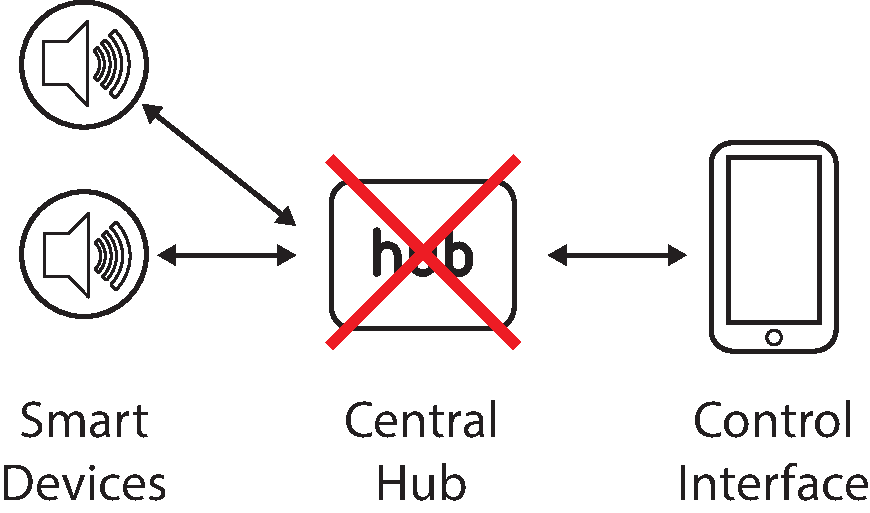
\includegraphics[width=\textwidth -200px]
     {graphics/smarthome-arthur.pdf}}
     \caption{\label{fig:use-case-2} Illustration of Arthur's use case.}
\end{figure}


\begin{quotation}\emph{\textbf{Use case: Sarah}\\
Sarah is interested in new technology, and as such she has a Smart Home system. Sarah lives on a farm far away from the city, where she has her job as a farmer on the family farm. Unfortunately, Sarah lives where her Internet connection is unstable. Her Smart Home system requires Internet connection to communicate between her devices, where the requests must go through a server. This use case is illustrated in \figref{fig:use-case-3}.}
\end{quotation}

\begin{figure}[H]
     \center{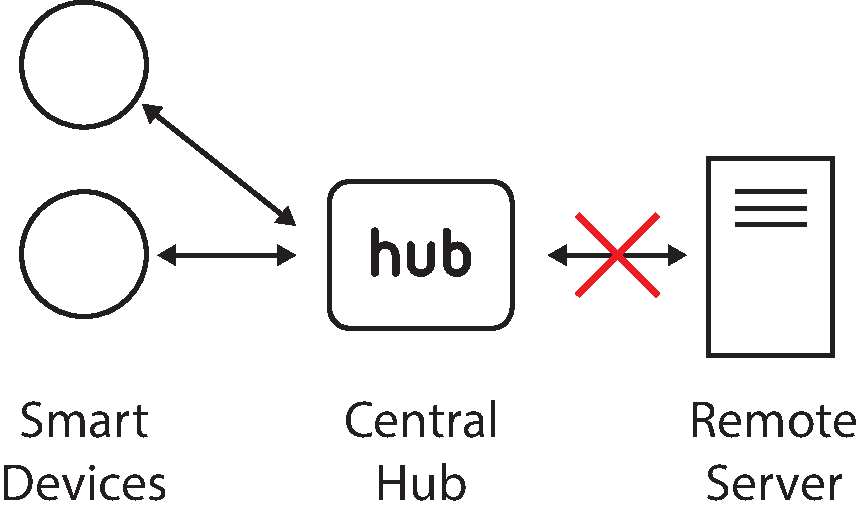
\includegraphics[width=\textwidth -200px]
     {graphics/smarthome-sarah2.pdf}}
     \caption{\label{fig:use-case-3} Illustration of Sarah's use case.}
\end{figure}